\begin{figure}[H]
    \centering
    \begin{minipage}{0.45\textwidth}
        \centering
        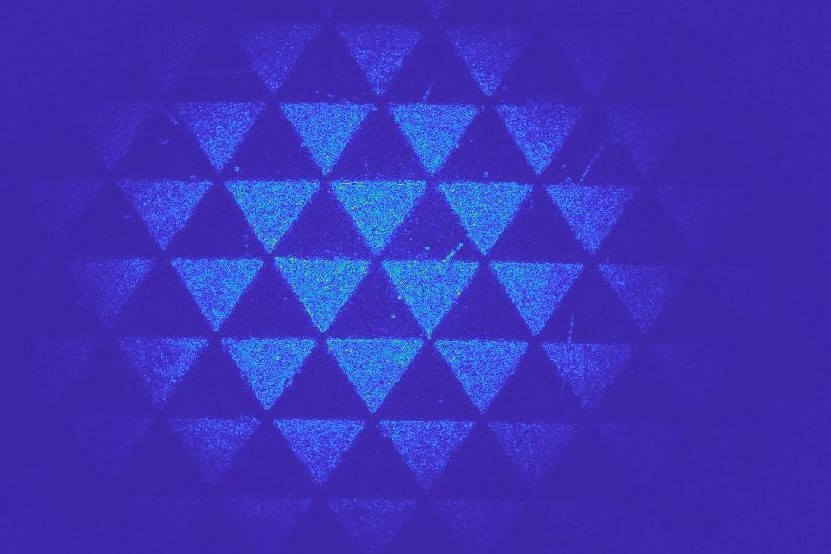
\includegraphics[ width = 0.95 \linewidth ]{figures/GradientImages/1549G.jpg}
        \caption{The gradient image of the captured inverse Fourier transform with no aperture}
    \end{minipage}%
    \hspace{0.75cm}
    \begin{minipage}{0.45\textwidth}
        \centering
        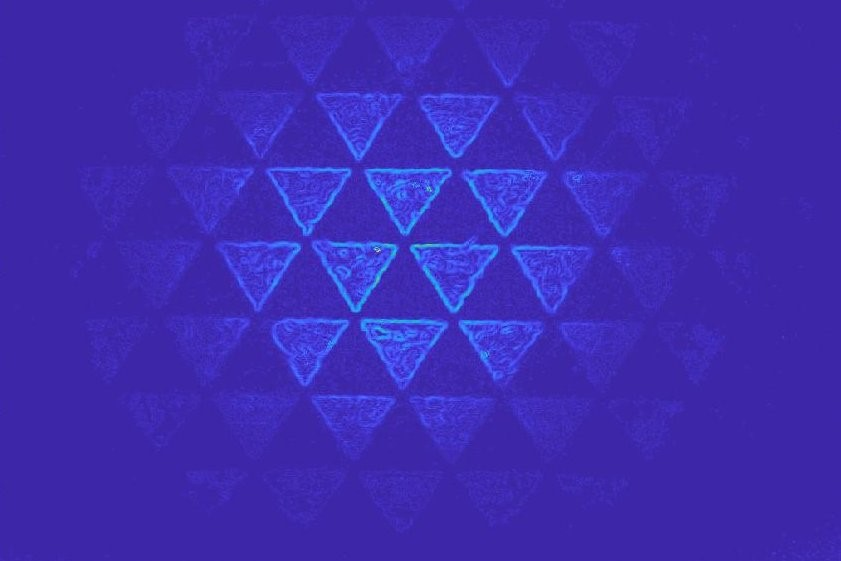
\includegraphics[ width = 0.95 \linewidth ]{figures/GradientImages/1548G.jpg}
        \caption{The gradient image of the captured inverse Fourier transform using the aperture with a diameter of $2.0 \ \si{mm}$}
    \end{minipage}%
    \vspace{1cm}
    \begin{minipage}{0.45\textwidth}
        \centering
        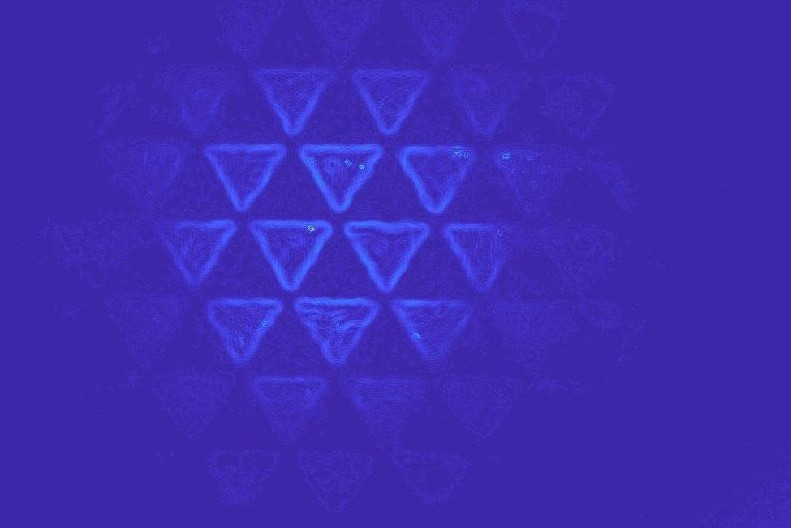
\includegraphics[ width = 0.95 \linewidth ]{figures/GradientImages/1547G.jpg}
        \caption{The gradient image of the captured inverse Fourier transform using the aperture with a diameter of $1.0 \ \si{mm}$}
    \end{minipage}%
    \hspace{0.75cm}
    \begin{minipage}{0.45\textwidth}
        \centering
        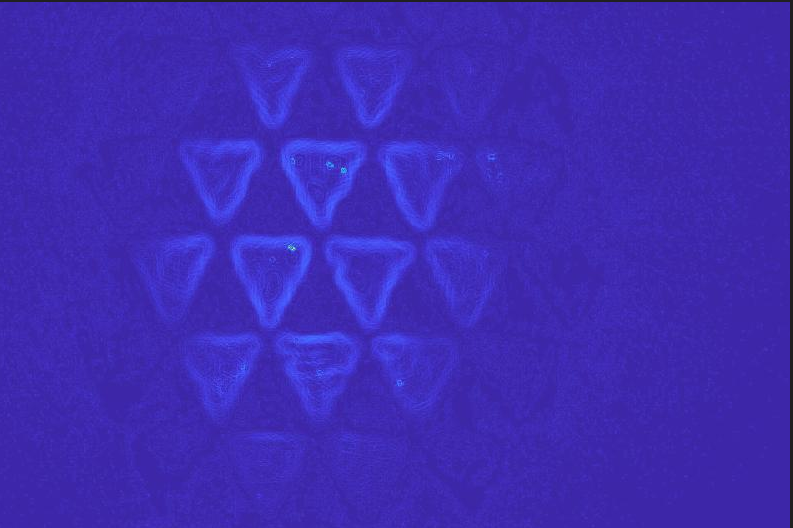
\includegraphics[ width = 0.95 \linewidth ]{figures/GradientImages/1546G.png}
        \caption{The gradient image of the captured inverse Fourier transform using the aperture with a diameter of $0.7 \ \si{mm}$}
    \end{minipage}%
    \vspace{1cm}
    \begin{minipage}{0.45\textwidth}
        \centering
        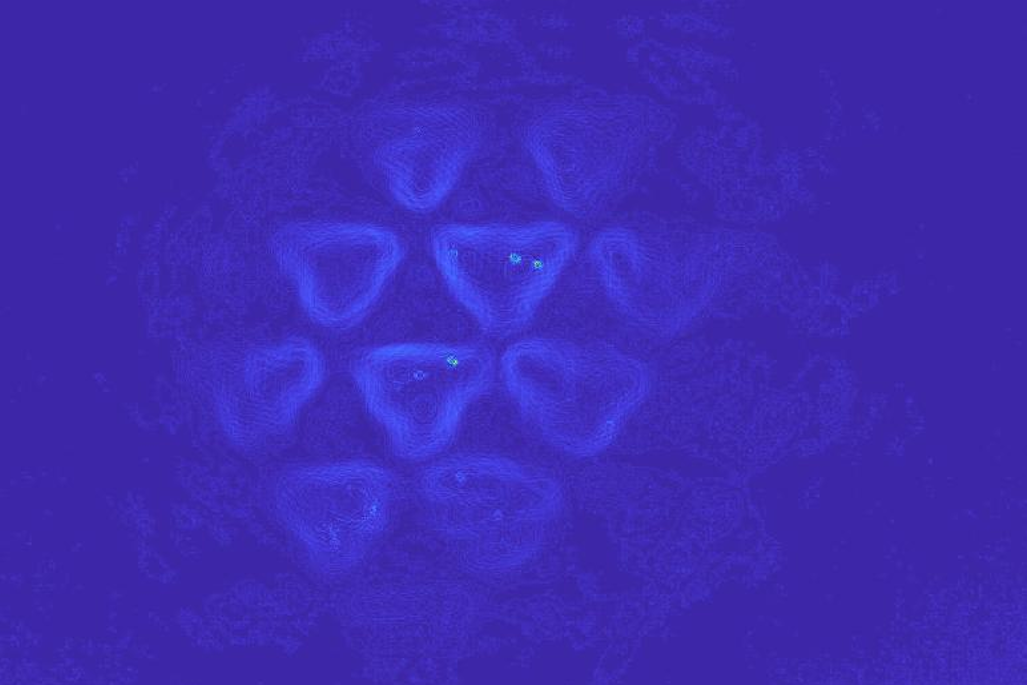
\includegraphics[ width = 0.95 \linewidth ]{figures/GradientImages/1545G.png}
        \caption{The gradient image of the captured inverse Fourier transform using the aperture with a diameter of $0.5 \ \si{mm}$}
    \end{minipage}%
    \hspace{0.75cm}
    \begin{minipage}{0.45\textwidth}
        \centering
        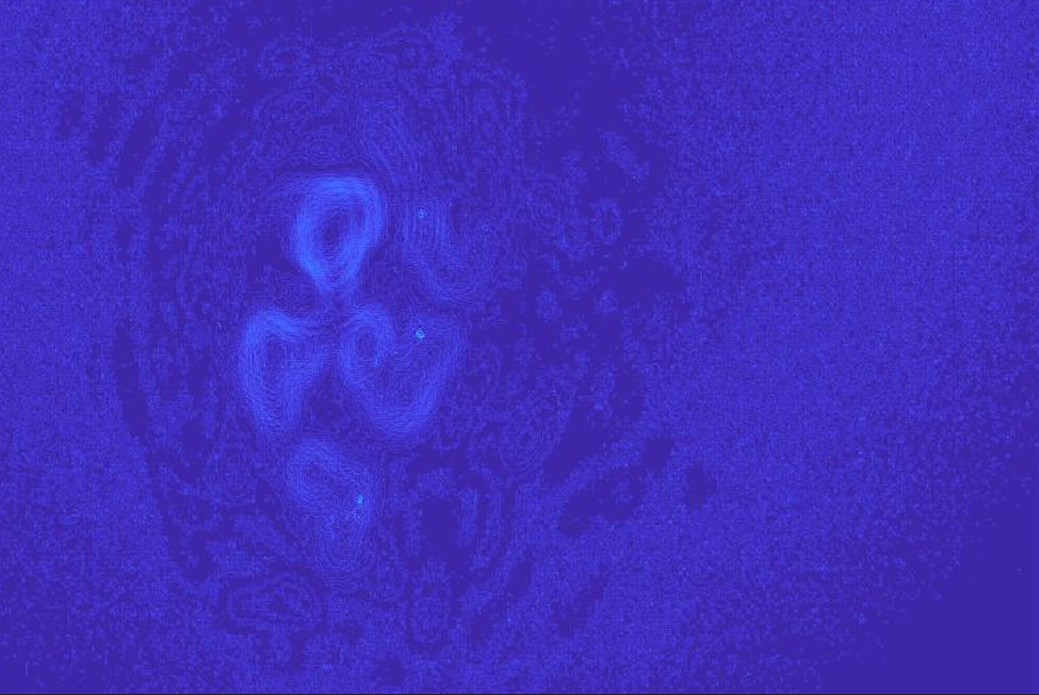
\includegraphics[ width = 0.95 \linewidth ]{figures/GradientImages/1544G.png}
        \caption{The gradient image of the captured inverse Fourier transform using the aperture with a diameter of $0.3 \ \si{mm}$}
    \end{minipage}%
\end{figure}